\chapter{Results \label{chap:results}}

\section{Survey}
The survey was completed by 12 people in total. Half of the participants have described themselves as well-acquainted with the area of games or animation. One person was not sure and the rest was not acquainted with that topic. However it appears that this is never strongly correlated (using Pearson correlation coefficient) to any of the other answers. It seems that having experience in games or animation does not significantly influence how the participants perceived the animations.

The participants were asked to decide whether the animations presented to them were realistic. The question was asked about each of the six scenes. The t-test was performed taking into account the answers about all the original scenes and the recreated scenes. The p-value of 0.7614 shows weak statistical significance of the result. The realism of the scenes was described on a one to five scale\footnote{The participants were asked to say whether they agree with the statement  `video X is realistic'. The answer was taken on a one to five scale where one means `strongly agree' and five means `strongly disagree'}, where the average score for both original and recreated scenes is about 3.1. These results show that animations generated by this project are no more realistic than the originals and that both original and recreated scenes are hardly realistic at all.
	
A similar set of questions was asked about the effectiveness in conveying emotions. The participants were asked to decide whether the animations correctly convey the feelings and emotions of the characters in the scene. This time the results yielded the p-value of 0.4657 showing a higher significance of the result. The participants' answers suggest that the animations reproduced by the software are slightly better at conveying feelings and emotions (the mean score of the recreated animations was by 0.3 (out of 5) better than the originals). These results show a very slight advantage of the recreated animations over the original ones.


\begin{figure}[H]
	\centerline{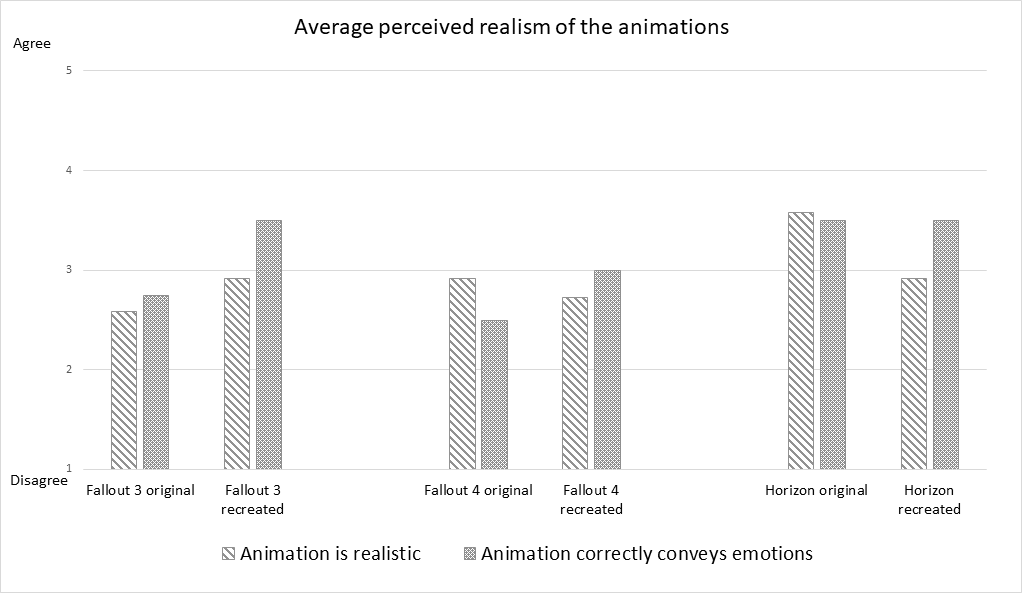
\includegraphics[width = 25em]{img/results/realism.png}}
	\caption{The addon UI}\label{fig:realism_graph}
\end{figure}












